\documentclass[border=7pt]{standalone}
\usepackage{tikz}

\begin{document}
  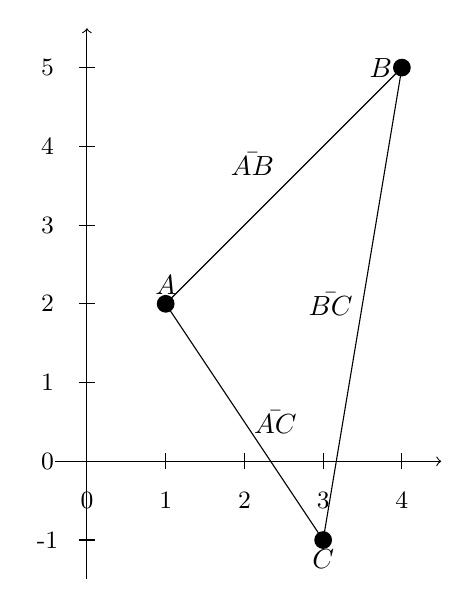
\begin{tikzpicture}
    \draw [->] (-0.4, 0) -- (4.5,0);
    \draw [->] (0,-1.5) -- (0,5.5);

    \foreach \x in {0,1,2,3,4} {
    \draw (\x,-0.5) node{\small\x};
    \draw (\x,-0.1) -- (\x,0.1);
    };

    \foreach \x in {-1,0,1,2,3,4,5} {
    \draw (-0.5,\x) node{\small\x};
    \draw (-0.1,\x) -- (0.1,\x);
    };

    \filldraw (1,2)circle(3pt) node [above] {$A$};
    \filldraw (4,5)circle(3pt)node [left] {$B$};
    \filldraw (3,-1)circle(3pt)node [below] {$C$};

    \draw[->] (1,2) -- (4,5) node[midway, above left] {$\bar{AB}$};
    \draw[->] (1,2) -- (3,-1) node[midway, right] {$\bar{AC}$};
    \draw[->] (4,5) -- (3,-1) node[midway, left] {$\bar{BC}$};

  \end{tikzpicture}
\end{document}
